% Artículo: predicción de llegadas de autobús con feeds que solo dan la posición y horarios interpolados.
% Compilar con: latexmk -pdf articulo.tex (pdflatex + biber). Las cifras de las tablas salen de resultados.py.
\documentclass[preprint,11pt,nonatbib]{elsarticle}

\usepackage[T1]{fontenc}
\usepackage[utf8]{inputenc}
\usepackage{lmodern}
\usepackage{microtype}
\setlength{\emergencystretch}{2em}
\usepackage{amsmath,amssymb,amsthm}
\usepackage{booktabs,tabularx}
\usepackage{xcolor}
\usepackage{tikz}
\usetikzlibrary{arrows.meta,positioning,decorations.pathreplacing}
\usepackage{pgfplots}
\pgfplotsset{compat=1.18}
\usepackage{algorithm}
\usepackage{algpseudocode}
\usepackage[hidelinks]{hyperref}
\makeatletter\let\c@author\relax\makeatother
\usepackage[style=authoryear,backend=biber,maxcitenames=2,uniquelist=false,giveninits=true,doi=true,url=false]{biblatex}
\addbibresource{referencias.bib}

\definecolor{ruta}{HTML}{01573C}
\definecolor{gps}{HTML}{C8102E}
\definecolor{gris}{HTML}{6B7280}

% Notación (la de la memoria técnica).
\newcommand{\Tpos}{T_{\mathrm{pos}}}
\newcommand{\tgps}{t_{\mathrm{gps}}}
\newcommand{\tref}{t_{\mathrm{ref}}}
\newcommand{\ETA}{\mathrm{ETA}}
\newcommand{\band}{\operatorname{band}}
\newcommand{\clamp}{\operatorname{clamp}}
\newcommand{\med}{\operatorname{med}}

% Pie de la primera página: preprint, versión y fecha (en lugar de «Preprint submitted to Elsevier»).
\makeatletter
\def\ps@pprintTitle{%
  \let\@oddhead\@empty
  \let\@evenhead\@empty
  \def\@oddfoot{\footnotesize\itshape Preprint, version 1.0 \hfill 7 November 2026}%
  \let\@evenfoot\@oddfoot}
\makeatother

\newtheorem{definition}{Definition}
\newtheorem{proposition}{Proposition}

\begin{document}

\begin{frontmatter}

\title{Predicting bus arrivals when the feed reports positions but not delays: a reproducible three-layer method
with an open reference implementation}

\author{Yeray Garrido\fnref{orcid}}
\fntext[orcid]{Independent researcher, Bilbao, Biscay, Spain. ORCID:
\href{https://orcid.org/0009-0008-0459-0294}{0009-0008-0459-0294}. E-mail:
\href{mailto:garridoparrayeraytx@gmail.com}{garridoparrayeraytx@gmail.com}. Code and data:
\url{https://github.com/Garridoparrayeray/bide-eta}.}

\begin{abstract}
Many public transport networks publish real-time vehicle positions but not delays, and many timetables give
intermediate stop times interpolated at constant speed rather than observed. Bizkaibus, the interurban bus network
of Biscay (Spain), has both properties: after the first hour of a trip, 85\% of buses pass a stop more than two
minutes before the published time. This paper specifies the arrival prediction method of the Bizkaibus+ app in
enough detail to reimplement it in any language. The method uses timetable differences instead of absolute times;
learns the actual travel time between consecutive stops by time band, as a median shrunk towards the all-day median
of the segment; and predicts from three layers with explicit abstention rules: the GPS position projected onto the
route, the last stop registered by the feed, and the timetable corrected trip by trip. It recalibrates itself daily,
adopting only changes that reduce the error on held-out data. In 9.1 million predictions over 23 days, checked
against the actual passage, the arrival shown is within $\pm2$~minutes in 92--96\% of cases when the bus is less than
three minutes away and in 67\% at ten to twenty minutes, against 23--25\% for the published timetable. Without any
live data, the corrected timetable alone doubles the accuracy of the published one. A reference implementation in
Python, test vectors with 407 checks produced by the production engine, a public evaluator that reproduces the production
histograms, and the learned tables and evaluation data are openly available.
\end{abstract}

\begin{keyword}
bus arrival prediction \sep real-time passenger information \sep GTFS \sep SIRI \sep robust estimation \sep
shrinkage \sep temporal validation \sep reproducibility
\end{keyword}

\end{frontmatter}

% =====================================================================================================================
\section{Introduction}
\label{sec:intro}

Real-time arrival information reduces both the time passengers wait at stops and the uncertainty of that wait, and
makes public transport more attractive \parencite{watkins2011,brakewood2019}. Producing it requires two inputs that
are not always available in the form a prediction method expects: a reliable reference schedule and a live estimate
of how far each vehicle is from it.

Bizkaibus, the interurban bus network of the province of Biscay in northern Spain, publishes both as open data: a
GTFS timetable \parencite{gtfs} and a SIRI Vehicle Monitoring feed \parencite{siri} with the GPS position and the
next stop of every vehicle in service. The feed, however, does not report vehicle delays, and the intermediate times
of the timetable are not operator commitments: they are interpolated linearly between the terminal times, at
constant speed along the route. Real buses are slower in towns and faster on highways, so the published intermediate
times drift further from the actual passage times as the trip progresses. Section~\ref{sec:drift} quantifies this drift:
over 169,308 observed stop passages, after the first hour of a trip 85\% of buses pass more than two minutes before
the published time, and the median passage is almost fourteen minutes early. A passenger who trusted the published
time and reached the stop two minutes beforehand would find that the bus had already gone in 52\% of cases.

This setting is not specific to Bizkaibus. Position-only feeds are common in automatic vehicle location systems, and
interpolated intermediate times are allowed by GTFS (\texttt{timepoint=0}) and widespread in regional networks. Under
these conditions, the absolute published time is a poor reference, and a method that predicts arrivals by adding a
delay to it inherits its error.

This paper describes the method that the Bizkaibus+ app\footnote{\url{https://www.bideplus.eus}. The app is
independent and is not affiliated with Bizkaibus, the Diputación Foral de Bizkaia or the operators of the service.}
uses to predict arrivals under these conditions. The aim is to make the method reusable: every rule is given with its
formula and constants, the evaluation protocol is specified so that it can be repeated on other data, and the
reference implementation, test vectors, evaluator and data are public. A longer technical report in Spanish
\parencite{garrido2026memoria} gives the measurements behind each constant, the history of each rule and the
evaluation of the first period used here. The contributions are:

\begin{enumerate}
  \item A representation of the vehicle state in \emph{timetable time}: the GPS position is projected onto the route
        and converted into the scheduled time at that point, so that predictions are built from timetable
        differences, which are reliable even when absolute times are not (Sections~\ref{sec:localisation}
        and~\ref{sec:differences}).
  \item A segment travel-time model learned from the feed itself, by time band and day type, with medians shrunk
        towards the all-day median of each segment, and a daily recalibration that adopts only changes that reduce
        the error on data not used to fit them: other vehicles, or later days for the per-trip correction
        (Sections~\ref{sec:segments} and~\ref{sec:learning}).
  \item A three-layer prediction with explicit abstention rules, which decides for each stop whether the vehicle
        position, the last registered stop or the corrected timetable gives the best available estimate, and states
        which one it used (Section~\ref{sec:layers}).
  \item An open, verifiable package: a reference implementation written only from the specification, test
        vectors with 407 checks produced by the production engine, an evaluator that reproduces the production
        histograms bin by bin, and the learned tables and evaluation data (Section~\ref{sec:reuse}).
\end{enumerate}

\noindent The rest of the paper reviews related work (Section~\ref{sec:related}), describes the data and the problem
(Section~\ref{sec:data}), presents the method (Section~\ref{sec:method}) and its evaluation
(Section~\ref{sec:evaluation}), explains how to reproduce and reuse the results (Section~\ref{sec:reuse}), discusses
limitations and open problems (Section~\ref{sec:discussion}) and concludes (Section~\ref{sec:conclusions}).

\begin{figure}[t]
\centering
\fbox{\begin{minipage}{0.94\textwidth}\small
\textbf{The method in plain language.} The timetable says, for every stop, when the bus should pass; its intermediate
times are wrong in absolute terms but consistent with each other. The method first asks \emph{where in the timetable}
the bus is: it projects the GPS position onto the route and reads the scheduled time at that point. A bus that is
physically where the timetable puts it at 10:20 is, in timetable terms, at 10:20, whatever the clock says. To predict
the arrival at a later stop, the method does not add a delay to the published time of that stop; it adds, to the
time at which the GPS position was taken, how long the remaining segments \emph{actually} take, as learned from weeks of observed passages.
When the GPS position is missing or unreliable, it uses the last stop that the feed reports the bus has passed; when
there is no live data at all, it uses the timetable corrected by what each trip usually does. Each prediction states
which of these three sources it comes from.
\end{minipage}}
\end{figure}

% =====================================================================================================================
\section{Related work}
\label{sec:related}

% Trabajo relacionado. Cada referencia está comprobada contra su DOI (Crossref) o su fuente primaria.

Bus arrival and travel time prediction has a long literature, recently reviewed by \textcite{kumar2025review} and, for
models based on artificial intelligence, by \textcite{singh2022review}. \textcite{moreiramatias2015survey} survey the
wider use of automatic vehicle location (AVL) data to evaluate and correct timetables.

\paragraph{Historical and segment-based methods} The simplest predictors average historical travel times, by route,
time of day or segment. \textcite{lin1999experimental} compared GPS-based algorithms for a rural service with long
headways that use the schedule and time-check stops, a setting close to interurban buses. Splitting a trip into
segments between consecutive stops and predicting each one is common: \textcite{gal2017journey} predict segment times
with a queueing-based snapshot predictor and machine learning, and observe that outliers are a problem, and
\textcite{mazloumi2010variability} show that travel-time variability depends strongly on the time window, which
motivates learning by time band. The method of this paper belongs to this family, with three specific choices: it
learns per segment and band rather than per line, it uses medians shrunk towards the all-day value of the segment,
and the live position resets the prediction at each update.

\paragraph{Kalman filters} Kalman filtering \parencite{kalman1960} updates a state, typically the vehicle's position
and speed or its delay, with each new observation. \textcite{cathey2003prescription} proposed a tracker–filter–predictor
framework for AVL data, \textcite{shalaby2004} combined AVL and passenger counts, \textcite{vanajakshi2009kalman}
applied a Kalman filter to buses in heterogeneous traffic, and \textcite{achar2020spatial} model the spatial
correlation between successive sections. Section~\ref{sec:evaluation} compares the method with two Kalman filters under
the same protocol.

\paragraph{Machine learning} Neural networks were applied to bus arrivals early on \parencite{chien2002}, and beat
historical and regression models on a Houston route \parencite{jeong2005}; support vector regression uses segment-level
inputs similar to ours \parencite{bin2006svm}. Recent work uses recurrent networks \parencite{pang2019rnn},
convolutional LSTMs that predict all links of a route at once \parencite{petersen2019convlstm}, graph attention
networks for sparse data \parencite{ma2022multiattention} and transformers trained on open data
\parencite{jeong2024battransformer}. In road-traffic forecasting, deep learning is not always the best technique and
strong simple baselines matter \parencite{manibardo2022deep}; our comparison points the same way.

\paragraph{Open feeds, published timetables and published predictions} Several studies use the open GTFS and real-time
feeds that agencies publish. \textcite{wessel2017retrospective} rebuild the timetable actually run from a public
vehicle-location feed, much as our ground truth is reconstructed from the feed, and \textcite{wessel2019accuracy} show
that published timetables overstate accessibility compared with what buses actually do. The accuracy of predictions
already shown to passengers has also been measured: \textcite{cats2016realtime} evaluated a deployed prediction scheme
in Stockholm and found that it underestimated the remaining wait, and \textcite{garciamaurino2024improving} correct the
systematic errors of agency predictions in Madrid and Paris using only data from public APIs, a third-party setting
close to ours. Real-time feeds have their own quality problems, such as latency \parencite{zhou2025latency}.

\paragraph{Shrinkage and robust estimation} Shrinking noisy estimates towards a common value reduces their mean squared
error \parencite{jamesstein1961,efronmorris1975}, and empirical Bayes estimation is standard in transport safety
\parencite{hauer2002empirical}. \textcite{woodard2017predicting} model travel-time distributions with a trip-level
effect and fall back to pooled parameters for links with few observations, a close analogue of our per-trip correction
and shrinkage. Median-based statistics are robust to outliers and incidents \parencite{huber1964,clark2002cleaning}.

\paragraph{Passenger value and evaluation} Real-time information improves satisfaction and perceived safety, and
inaccurate predictions reduce ridership \parencite{gooze2013benefits,brakewood2019}; its value depends on the quality of
the predictions \parencite{liu2020waiting} and is greatest on low-frequency services \parencite{rahman2013users}, such
as interurban buses. Evaluating forecasts requires keeping the future out of the past: rolling-origin, out-of-sample
evaluation \parencite{tashman2000outofsample}, order-preserving validation for non-stationary series
\parencite{cerqueira2020evaluating} and strict separation of the data used to learn and to predict
\parencite{kaufman2012leakage}. The method's daily recalibration and its day-by-day evaluation follow these principles.


% =====================================================================================================================
\section{Data and problem setting}
\label{sec:data}

\subsection{Timetable}
The timetable is the Bizkaibus GTFS feed published through the Spanish National Access Point for transport
\parencite{nap}. It contains about 100 lines. Every line has an identifier (\texttt{route\_id}, e.g.\ \texttt{651})
and a public name (\texttt{route\_short\_name}, e.g.\ \texttt{A0651}). Intermediate stops carry
\texttt{timepoint=0}: their times are interpolated linearly with distance between the terminal times.

\subsection{Live feed}
The SIRI Vehicle Monitoring feed is a public XML document regenerated about once a minute, with about 250 vehicles at
peak times. For every vehicle it gives the trip reference (equal to a GTFS \texttt{trip\_id}), the vehicle
identifier, the GPS position and its time, and the order of the next stop in the trip. It does not report the delay.
From 23:58 to 05:00 the feed repeats the vehicles seen before midnight with their old times; these entries carry no
time of the new day and are ignored (Section~\ref{sec:practical}).

\subsection{Why the timetable is not an absolute reference}
\label{sec:drift}

Figure~\ref{fig:drift} shows the deviation of the actual passage from the published time over 169,308 observed stop
passages, as a function of the scheduled time elapsed since departure from the terminal. Near the terminal, buses are
slightly late (median $+1.3$~min in the first ten minutes). From there on they are increasingly early: half an hour
after departure, half of the passages occur more than two minutes before the published time, and after one hour 85\%
do, the median passage being almost fourteen minutes early. Only a quarter of all passages fall within
$\pm2$~minutes of the published time. These figures are not a judgement on the punctuality of the service, since the
intermediate times are not operator commitments; they are, however, the times that a passenger sees in any
application that does not correct them.

\begin{figure}[t]
\centering
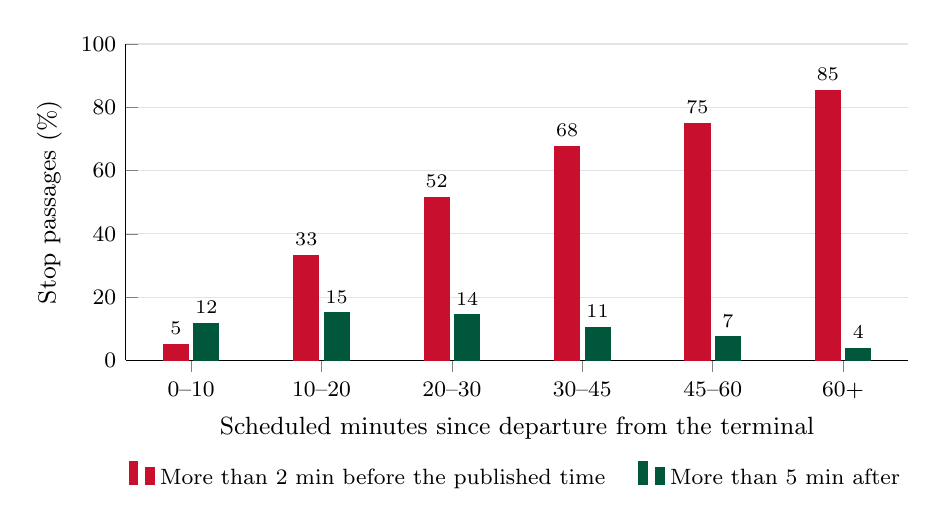
\begin{tikzpicture}
\begin{axis}[
  width=0.95\textwidth, height=5.6cm,
  ybar, bar width=9pt,
  symbolic x coords={0--10,10--20,20--30,30--45,45--60,60+},
  xtick=data,
  xlabel={Scheduled minutes since departure from the terminal},
  ylabel={Stop passages (\%)},
  ymin=0, ymax=100,
  axis lines*=left, ymajorgrids, grid style={gris!20},
  tick label style={font=\footnotesize}, label style={font=\small},
  legend style={font=\footnotesize,draw=none,fill=none,at={(0.5,-0.3)},anchor=north,legend columns=2,/tikz/every even column/.append style={column sep=1em}},
  nodes near coords, every node near coord/.append style={font=\scriptsize,color=black},
  nodes near coords style={/pgf/number format/fixed,/pgf/number format/precision=0}]
\addplot[fill=gps,draw=gps] coordinates {(0--10,5.0) (10--20,33.3) (20--30,51.5) (30--45,67.6) (45--60,74.8) (60+,85.4)};
\addlegendentry{More than 2 min before the published time}
\addplot[fill=ruta,draw=ruta] coordinates {(0--10,11.8) (10--20,15.0) (20--30,14.4) (30--45,10.5) (45--60,7.4) (60+,3.7)};
\addlegendentry{More than 5 min after}
\end{axis}
\end{tikzpicture}
\caption{Deviation of the actual passage from the published time, by scheduled time since departure (169,308 stop
passages). Because the timetable assumes constant speed and buses run faster on open-road sections, they pass
increasingly early as the trip progresses.}
\label{fig:drift}
\end{figure}

% =====================================================================================================================
\section{Method}
\label{sec:method}

% Sección del método: localización, modelo del tiempo por tramo, tres capas, aprendizaje y casos prácticos.
% Cada regla coincide con referencia/referencia.py y con las 407 comprobaciones de los vectores de prueba.

\subsection{Notation and conventions}
\label{sec:notation}

A trip $J$ of line $\ell$ visits stops $p_1,\dots,p_N$. Stop $p_i$ has order $i$, coordinates, published arrival and
departure times $a_i\le d_i$ and, when the trip has a shape, a distance $s_i$ along it (\texttt{shape\_dist\_traveled}).
Times are seconds since midnight (Europe/Madrid) of the trip's service day $D$ and, as in GTFS, may exceed 86,400
(26:10 is 94,200~s). Segment $i$ of $J$ is the pair of consecutive stops $\kappa_i=(p_i,p_{i+1})$; a segment $\kappa$
is identified by its two stop identifiers, so that all lines running it share what is learned about it. Its scheduled
duration is $h_i=a_{i+1}-a_i$ and, when both distances are known, its length is $L_i=s_{i+1}-s_i$.

Each entry $e$ of the live feed carries a trip reference, a GTFS \texttt{trip\_id} that also encodes the line, the
trip number and the departure $d^{\mathrm{feed}}$ of the trip in seconds (\texttt{trp\_A0651\_737\_ABC1\_28500} gives
line 651, trip number 737 and $d^{\mathrm{feed}}=28{,}500$; entries whose reference does not have this form are
ignored); a vehicle identifier; and, when present, the order $n$ of the next stop (\texttt{Order}, or
\texttt{VisitNumber}), a GPS position with its time $\tgps$ (\texttt{LocationRecordedAtTime}, or
\texttt{RecordedAtTime} if absent) and the time $t_{\mathrm{rec}}$ of the record (\texttt{RecordedAtTime}). Feed
times are converted to local time; a time whose date is not the current day is discarded, and so is a position whose
time is discarded. $t_{\mathrm{now}}$ is the current time.

A \emph{time band} $\band(D,t)$ is one of twelve: the day type of $D$ (weekend on Saturday and Sunday, weekday
otherwise) combined with one of six periods of the hour $\lfloor t/3600\rfloor\bmod24$, starting at 0, 6, 9, 13, 16
and 20~h; 26:10 on a Friday thus falls in the Friday band that starts at 0~h. Four conventions are needed to
reproduce every number. $\operatorname{rnd}$ rounds halves away from zero, and
$\operatorname{rnd}_3(x)=\operatorname{rnd}(1000x)/1000$. $Q_\alpha(x)=x_{(\lfloor\alpha(|x|-1)\rfloor)}$ is the
percentile $\alpha$ of the sorted values $x_{(0)}\le\dots\le x_{(|x|-1)}$, without interpolation, and
$\med=Q_{0.5}$ is the low median. $\clamp(x,x_{\min},x_{\max})=\max(x_{\min},\min(x_{\max},x))$. Line numbers are
written as in the timetable, without leading zeros, also in the keys of the learned tables: the feed writes
\texttt{A0651} for line \texttt{651}. Appendix~\ref{app:constants} lists every constant.

\subsection{Matching and localisation}
\label{sec:localisation}

\paragraph{Matching} Calendar variants of the same trip are merged when the timetable database is built, and a table
of aliases maps every original \texttt{trip\_id} to its merged trip. A trip $J$ is matched to the first feed entry
whose reference is an alias of $J$; on the live feed every vehicle was matched this way. Only if there is none is the
fallback used: among the entries with the line and trip number of $J$ whose reference is not an alias of another trip
(an entry matched exactly is never reused), the one whose $d^{\mathrm{feed}}$ is closest to $d_1$ is taken, provided
$|d^{\mathrm{feed}}-d_1|\le180$~s (the first one on a tie). Otherwise the trip has no feed entry.

\paragraph{Projection} All localisation rests on projecting the GPS position onto a straight segment $AB$ in a local
equirectangular plane centred on the vehicle. With $(\varphi,\lambda)$ the latitude and longitude of the vehicle in
degrees, a point of latitude $\varphi'$ and longitude $\lambda'$ has planar coordinates
$\big((\lambda'-\lambda)\cos\varphi\cdot111{,}320,\ (\varphi'-\varphi)\cdot111{,}320\big)$ in metres. With $\mathbf a$
and $\mathbf b$ the planar coordinates of $A$ and $B$ and $\mathbf u=\mathbf b-\mathbf a$,
\begin{equation}
f=\clamp\!\Big(-\frac{\mathbf a\cdot\mathbf u}{\|\mathbf u\|^2},0,1\Big),\qquad d_\perp=\|\mathbf a+f\mathbf u\|,
\label{eq:projection}
\end{equation}
with $f=0$ if $A=B$: $f$ is the fraction of the segment from $A$ to the point closest to the vehicle, $d_\perp$ the
distance to that point and $\|\mathbf u\|$ the length of the segment. The distance from the vehicle to a stop is
computed in the same way, with the cosine of the stop's latitude.

\paragraph{Search window} The declared next stop bounds where the vehicle can be. The search covers segments $i_{\min}$
to $i_{\max}$ with
\begin{equation}
i_{\min}=\max(1,n-3),\qquad i_{\max}=\min(N-1,n+2),
\label{eq:window}
\end{equation}
that is, stops $p_{n-3}$ to $p_{n+3}$ where the trip has them. Looking back covers a feed that changes the next stop
too early, while the bus is still before $p_{n-1}$; looking ahead covers one that changes it late, when the bus is
already past $p_n$.

\paragraph{With a shape} This method is used when the trip has a shape and every stop of the window has a distance.
Every pair of consecutive shape points $A,B$, with distances $s_A$ and $s_B$ along the shape, such that
$s_B\ge s_{i_{\min}}$ and $s_A\le s_{i_{\max}+1}$ gives a candidate position along the route,
$s^\ast=s_A+f(s_B-s_A)$. Candidates with $s^\ast\le s_n+100$~m are \emph{expected}, the rest \emph{beyond}; each group
keeps its candidate with the smallest $d_\perp$ (the first one on a tie). The expected candidate wins unless there is
none or the beyond one is more than 20~m closer, which resolves routes that pass twice along the same street in
favour of the declared next stop. The position is valid if the chosen candidate has $d_\perp\le50$~m. Then $s^\ast$
is clamped to $[s_{i_{\min}},s_{i_{\max}+1}]$, $i$ is the first segment of the window with $s^\ast\le s_{i+1}$, and
the scheduled time at the vehicle's position is
\begin{equation}
\Tpos=\operatorname{rnd}\big(d_i+f_i(a_{i+1}-d_i)\big),\qquad f_i=\clamp\Big(\frac{s^\ast-s_i}{s_{i+1}-s_i},0,1\Big),
\label{eq:tpos}
\end{equation}
with $f_i=0$ if $s_{i+1}=s_i$. The time is interpolated from the departure at $p_i$, not the arrival, since within a
segment the vehicle is moving.

\paragraph{Without a shape} Otherwise the vehicle is projected onto the straight segments $p_ip_{i+1}$ of the window
and the closest one is kept (the first one on a tie). The position is valid if
$d_\perp\le\max(150~\text{m},\,0.15\,\|\mathbf u\|)$, a corridor that widens with the straight-line length
$\|\mathbf u\|$ of that segment, and then $\Tpos=\operatorname{rnd}\big(d_i+f(a_{i+1}-d_i)\big)$, with $f$ from
Eq.~\eqref{eq:projection}. Because the timetable database measures stop distances on the shape when a network does
not publish them, this case only remains for trips with no shape at all.

\paragraph{Conditions} A position requires the entry to have coordinates, $\tgps$ and $n$, the data to be recent
($t_{\mathrm{now}}-\tgps\le600$~s) and the trip to have at least two stops. If the trip has started or is about to
($\tgps\ge d_1-60$~s), it also requires $n$ to be the order of a stop of the trip, the projection to be valid and the
GPS not to contradict the registered stop (the cross-check of Section~\ref{sec:layers}). If $\tgps<d_1-60$~s, the
only possible position is at the first stop: a vehicle within 150~m of $p_1$ and with $d_1-\tgps\le3{,}600$~s is
placed there, with $\Tpos=\min(a_1,d_1)$ and $\tgps$ replaced by $d_1$, because it has not travelled at all and will
leave at its time at the earliest. A position at the first stop never gives a passage and is not learned from.

\paragraph{Shapes that do not match their stops} The method depends on the shape and the stop distances agreeing. In
the Bizkaibus timetable of 3 November 2026, 55 of the 440 shapes used by trips were drawn from the last stop to the
first (670 of 6,130 merged trips, on 25 lines), and in 1,417 trips some stop was more than 200~m from the point its
distance indicated. The timetable database therefore reverses a shape (it reverses the order of the points and
replaces each distance $s$ by $s_{\max}-s$) when, in most of its trips, the distance from the first stop to the last
shape point plus that from the last stop to the first point is smaller than the distance from the first stop to the
first point plus that from the last stop to the last point. If a shape was reversed, or some stop of a trip is more
than 100~m from the point its distance indicates, all the stop distances of the trip are measured again by projecting
each stop onto the shape from the previous one, searching at most three times the straight-line distance between the
two stops plus 500~m; where the shape passes twice near a stop, the first pass wins unless the second is 30~m closer.
After the correction, 26 trips kept a stop more than 200~m away.

\subsection{Why timetable differences}
\label{sec:differences}

Let $T(s)$ be the time at which the timetable places the vehicle at the point $s$ of the route, $R(s)$ the real time
and $\Delta(s)=R(s)-T(s)$ the offset. The vehicle was seen at $s_p$ at $\tgps=R(s_p)$, and the stop of interest is at
$s_d>s_p$.

\begin{proposition}
\label{prop:differences}
The published time $\hat R_{\mathrm{tt}}=T(s_d)$ has error $R(s_d)-\hat R_{\mathrm{tt}}=\Delta(s_d)$. The
\emph{difference} estimate $\hat R_{\mathrm{dif}}=\tgps+T(s_d)-T(s_p)$ has error $\Delta(s_d)-\Delta(s_p)$. More
generally, for any estimate $\hat E$ of the real travel time from $s_p$ to $s_d$, $\hat R=\tgps+\hat E$ has error
$\big(R(s_d)-R(s_p)\big)-\hat E$, which does not depend on $\Delta(s_p)$.
\end{proposition}
\begin{proof}
Since $\tgps=T(s_p)+\Delta(s_p)$, $R(s_d)-\tgps-T(s_d)+T(s_p)=\Delta(s_d)-\Delta(s_p)$; the last statement is
$R(s_d)-\tgps-\hat E=\big(R(s_d)-R(s_p)\big)-\hat E$.
\end{proof}

\noindent Three consequences guide the method. The delay accumulated before $s_p$ does not matter: a bus twenty
minutes late makes the published time wrong by twenty minutes and the difference estimate by almost nothing. The
\emph{profile} of the timetable does matter: with interpolated intermediate times, $T(s_d)-T(s_p)$ can be twice the
real time on a highway, so it is replaced by a learned estimate of the real travel time. And the error grows with the
number of segments between the vehicle and the stop, as each adds its own variation.

\subsection{Segment travel times}
\label{sec:segments}

\paragraph{Samples} Let $P_i$ be the real passage of a vehicle at stop $p_i$, reconstructed from its GPS positions as
described in Section~\ref{sec:learning}. Two consecutive passages $P_i<P_{i+1}$ of the same \emph{track} (one vehicle
on one trip on one date) give a segment sample: the real travel time $P_{i+1}-P_i$, rounded to 0.1~s, in the band
$\band(D,\lfloor P_i\rfloor)$ of the moment the vehicle entered the segment. For a segment $\kappa$ and a group $g$ (a
band, or the group $\mathtt{all}$ of every band), each track contributes a single value (its last sample in file
order), so that a bus seen many times does not weigh more than one seen once; $Y_{\kappa,g}$ is the list of these
values and $n_{\kappa,g}$ the number of tracks.

\paragraph{Shrunk medians} A segment is considered only if $n_{\kappa,\mathtt{all}}\ge2$. With
$m_\kappa=\med(Y_{\kappa,\mathtt{all}})$ and, for every band $b$ with $n_{\kappa,b}\ge2$,
$m_{\kappa,b}=\med(Y_{\kappa,b})$, the learned time in band $b$ is
\begin{equation}
\tau_{\kappa,b}=\operatorname{rnd}\!\left(\frac{n_{\kappa,b}\,m_{\kappa,b}+n_0\,m_\kappa}{n_{\kappa,b}+n_0}\right),\qquad n_0=5.
\label{eq:shrinkage}
\end{equation}
The any-time value $\tau_{\kappa,\mathtt{all}}=\operatorname{rnd}(m_\kappa)$ is stored only if the segment has samples
in at least two bands; otherwise it would be one band's value applied to bands with no measurement. The learned time
of $\kappa$ in band $b$ is $\tau(\kappa,b)=\tau_{\kappa,b}$ if it is stored, otherwise $\tau_{\kappa,\mathtt{all}}$
if it is stored; $\kappa$ is \emph{learned} in $b$ if $\tau(\kappa,b)$ is defined. Equation~\eqref{eq:shrinkage} has
the form of the posterior mean of a hierarchical normal model \parencite{gelman2013,efronmorris1975}, with $n_0$ in
the role of the ratio of within-band to between-band variance; the method uses medians for robustness
\parencite{huber1964} and fixes $n_0$ by validation.

\begin{proposition}
\label{prop:shrinkage}
Let $\hat\eta_b$ be an unbiased estimator of $\eta_b$ with variance $\sigma^2/n_b$, and $\mu$ a fixed value with
$\eta_b-\mu=\beta$. The shrunk estimator $\tilde\eta_b=\omega\hat\eta_b+(1-\omega)\mu$, with
$\omega=n_b/(n_b+n_0)$, has mean squared error $\omega^2\sigma^2/n_b+(1-\omega)^2\beta^2$, which is smaller than that
of $\hat\eta_b$ whenever $\beta^2<\sigma^2(2n_b+n_0)/(n_b\,n_0)$. The bound grows as $n_b$ decreases.
\end{proposition}
\begin{proof}
$\tilde\eta_b-\eta_b=\omega(\hat\eta_b-\eta_b)-(1-\omega)\beta$, a zero-mean term with variance
$\omega^2\sigma^2/n_b$ plus a constant. The inequality is $(1-\omega)^2\beta^2<(1-\omega^2)\sigma^2/n_b$, i.e.\
$\beta^2<\frac{1+\omega}{1-\omega}\frac{\sigma^2}{n_b}$, and $\frac{1+\omega}{1-\omega}=\frac{2n_b+n_0}{n_0}$.
\end{proof}

\noindent Shrinkage therefore helps bands with few tracks and barely changes bands with many, while too large an $n_0$
erases real differences between bands; Section~\ref{sec:evaluation} shows both effects. The proposition assumes an
unbiased estimator and a fixed $\mu$, whereas the method uses low medians and estimates $\mu$ ($m_\kappa$) from data
that include the band's own tracks: it is a heuristic justification, and the value of $n_0$ is decided by
measurement.

\paragraph{Length fallback} A segment without a learned time is estimated from its length, because the error of an
interpolated timetable depends mostly on it: short urban segments take about the scheduled time and long interurban
ones much less. A length $L$ falls in bucket $c(L)$, the number of the cuts 300, 600, 1,000, 1,500 and 3,000~m that
do not exceed $L$ (six buckets). Every segment sample with scheduled duration $h_i>0$ and known length (at
calibration, the low median of $s_{i+1}-s_i$ over the timetable trips that run the segment) gives a ratio of real to
scheduled time. For each bucket $c$ and group $g$, $r_{c,g}$ is $\operatorname{rnd}_3$ of the low median of all these
ratios (not one per track), and is stored if there are at least 20. For an unlearned segment $i$ of the trip,
$\tau^{\mathrm L}(h_i,L_i,b)=\clamp(r,0.3,1.5)\cdot h_i$, with $r=r_{c(L_i),b}$ if it is stored, otherwise
$r_{c(L_i),\mathtt{all}}$; $\tau^{\mathrm L}$ is undefined if $L_i$ is unknown or not positive, or if neither ratio
exists. On 31 October 2026 the ratio of the group $\mathtt{all}$ fell monotonically from 0.987 below 300~m to 0.534
at 3~km or more.

\paragraph{Pace factor} The last resort, and the only model when a network starts with no learned segments, is a pace
factor by band and, with enough data, by line and band: $k(\ell,D,t)=\clamp(\hat k,0.6,1.2)$, where
$\hat k=k_{\ell,b}$ if it exists, otherwise $k_b$ if it exists, otherwise 1, and $b=\band(D,t)$. A \emph{pace sample}
(Section~\ref{sec:learning}) records, for a vehicle with a position and a later stop of its trip, the scheduled
remaining time $H$ and the real remaining time $Z$. Each track contributes the ratio $\rho=\sum Z/\sum H$ over its pace
samples and, for a set of $n_\rho$ tracks (those of a band, or of a line in a band),
\begin{equation}
k=\operatorname{rnd}_3\Big(\clamp\big(1+(\tilde\rho-1)\tfrac{n_\rho}{n_\rho+10},\,0.6,\,1.2\big)\Big),
\label{eq:pace}
\end{equation}
with $\tilde\rho$ the low median of their ratios: a shrinkage towards the timetable as it is. $k_b$ needs eight
tracks, and $k_{\ell,b}$ 25 tracks and five different vehicles in the band.

\paragraph{Expected time} For segment $i$ of $J$, with band $b$ and pace factor $k$, the segment time $\tau_i$ is the
first defined value of the cascade $\tau(\kappa_i,b)$, $\tau^{\mathrm L}(h_i,L_i,b)$, $k\,h_i$. The expected real time
between two scheduled instants $t_0\le t_1$ of the trip is
\begin{gather}
E(J,t_0,t_1,b,k)=\sum_{i\in I(t_0,t_1)}\max(0,w_i)\,\tau_i,\label{eq:expected}\\
w_i=\frac{\min(a_{i+1},t_1)-\max(a_i,t_0)}{a_{i+1}-a_i},\nonumber
\end{gather}
with $w_i=1$ when $a_{i+1}=a_i$. $I(t_0,t_1)$ walks the segments in order, skipping those with $a_{i+1}\le t_0$ and
stopping at the first with $a_i\ge t_1$. Within a segment the vehicle advances at the timetable's pace; between
segments, at the learned one. If no segment table exists, $E=k\,(t_1-t_0)$. The whole path uses a single band $b$ and
pace factor $k$: in layers 1 and 2, those of the observation time; in layer 3, those of the midpoint between $d_1$ and
the published time of the target stop (Section~\ref{sec:layers}).

\subsection{Three-layer prediction}
\label{sec:layers}

The prediction for a \emph{row}, one departure of trip $J$ from a target stop of order $q$ and published time
$a_{\mathrm{dest}}$, uses the most reliable source available and says which one it used. Each layer abstains under
explicit conditions, and when none can support an estimate the published time is shown as such. A row has a state
(Table~\ref{tab:states}), an estimated arrival $\ETA$ and a delay $\delta$ in seconds. Only rows computed from a
position (layer 1) assert a delay; the others carry $\delta=0$. A delay of \emph{none} means that no delay is
asserted.

\begin{table}[t]
\centering
\caption{States of a prediction.}
\label{tab:states}
\small
\begin{tabularx}{\textwidth}{@{}lX@{}}
\toprule
State & Meaning \\
\midrule
\texttt{live} & Layer 1: the GPS places the vehicle on the route, or at its first stop before departure; a delay can be
asserted. \\
\texttt{estimated} & Layer 2 or 3: an estimate without live tracking; no delay is asserted. \\
\texttt{departed} & The vehicle has already passed the stop. \\
\texttt{likely\_departed} & No usable vehicle data, and the corrected timetable places the passage more than ten
minutes ago and at least ten minutes before the published time; or, with a position, the computed arrival passed more
than three minutes ago without the feed or the GPS confirming the passage. \\
\texttt{scheduled} & No layer can support an estimate: the published time, labelled as such. \\
\bottomrule
\end{tabularx}
\end{table}

\paragraph{Layer 1: GPS position} With a position, $b=\band(D,\tgps)$, $k=k(\ell,D,\tgps)$ and, if
$a_{\mathrm{dest}}\ge\Tpos$,
\begin{equation}
\ETA=\operatorname{rnd}\big(\tgps+E(J,\Tpos,a_{\mathrm{dest}},b,k)\big),\qquad \delta=\ETA-a_{\mathrm{dest}}.
\label{eq:layer1}
\end{equation}
If $a_{\mathrm{dest}}<\Tpos$, the timetable places the stop behind the vehicle: unless the row is \texttt{departed}
(see \emph{Passed stops} below), $\ETA=\tgps-(\Tpos-a_{\mathrm{dest}})$ and $\delta=\tgps-\Tpos$. The prediction
starts from $\tgps$, not from $t_{\mathrm{now}}$: the feed arrives about a minute after the position was taken, and
adding the remaining time to $t_{\mathrm{now}}$ would shift every arrival by that lag. A vehicle waiting at its first
stop is treated after layer 3.

\paragraph{Layer 2: registered stop} Many entries carry the next stop and the time of the record but no usable
position. The feed then says that the vehicle has left $p_{n-1}$ and is heading to $p_n$, at the reference time
$\tref$ ($\tgps$ if it exists, otherwise $t_{\mathrm{rec}}$). The entry has a \emph{registered stop} if $n\ge2$, the
trip has stops of orders $n-1$ and $n$, $t_{\mathrm{now}}-\tref\le600$~s, $\tref\ge d_1-60$~s, and the segment is
short ($a_n-a_{n-1}\le1{,}200$~s). The vehicle is then assumed to be half-way along it: with $b=\band(D,\tref)$ and
$k=k(\ell,D,\tref)$, for a target stop with $q\ge n$,
\begin{equation}
\theta=\operatorname{rnd}\big(\tfrac12E(J,a_{n-1},a_n,b,k)\big),\qquad
\ETA=\operatorname{rnd}\big(\tref+\theta+E(J,a_n,a_{\mathrm{dest}},b,k)\big),
\label{eq:layer2}
\end{equation}
with the last term zero if $a_{\mathrm{dest}}\le a_n$. Half is the expected remaining fraction if the observation
instant is independent of the position; shares from 0.35 to 0.65 were tested and 0.5 was best. On longer segments the
uncertainty of ``half-way'' is too large and the layer abstains. Layer-2 predictions are shown as \texttt{estimated},
without a delay; an arrival more than 120~s in the past is no longer credible, and the row goes to layer 3.

\paragraph{Cross-check} When an entry has both a position and a registered stop, their estimates of the offset should
agree. With $\delta_{\mathrm{pos}}=\tgps-\Tpos$ and $\delta_{\mathrm{reg}}=\tref+\theta-a_n$, if
$a_n-a_{n-1}\le360$~s and $|\delta_{\mathrm{pos}}-\delta_{\mathrm{reg}}|>360$~s, one of them is wrong and there is no
way to know which: the entry loses both, and the rows of its trip go to layer 3. The position, with this check, is
evaluated before any use of the registered stop.

\paragraph{Layer 3: corrected timetable} With no reliable vehicle data, the best estimate is a vehicle that leaves the
first stop a little after its time and runs every segment in its learned time. Let $D'$ be the service day $D$, except
on a weekday holiday (a weekday on which the timetable runs, by exception, a Sunday-only calendar), when $D'$ is the
Sunday of that week; a holiday thus uses weekend bands, pace factors and per-trip corrections. If a segment table
exists and $a_{\mathrm{dest}}>d_1$, with $b=\band(D',t_{\mathrm{mid}})$ and $k=k(\ell,D',t_{\mathrm{mid}})$ taken at
the midpoint $t_{\mathrm{mid}}=\lfloor(d_1+a_{\mathrm{dest}})/2\rfloor$, the corrected timetable is
\begin{equation}
C=d_1+60+\operatorname{rnd}\big(E(J,d_1-1,a_{\mathrm{dest}},b,k)\big)+\operatorname{rnd}(\gamma_v),
\label{eq:layer3}
\end{equation}
where $\gamma_v$ is the per-trip correction defined below (0 without a correction table). The 60~s reflect that buses
leave the first stop slightly late, and starting at $d_1-1$ includes segments of zero scheduled duration at the start
of the trip. If $C\ge t_{\mathrm{now}}$, the row is \texttt{estimated} with $\ETA=C$. If $C<t_{\mathrm{now}}-600$~s,
$a_{\mathrm{dest}}-C\ge600$~s and the segments of $I(d_1-1,a_{\mathrm{dest}})$ learned in band $b$ make up at least
80\% of the total scheduled duration of that path, the corrected timetable says with confidence that the bus passed
more than ten minutes ago, and at least ten minutes before its published time: the row is \texttt{likely\_departed},
shown with $\ETA=a_{\mathrm{dest}}$ at the end of the list. Otherwise, and whenever there is no segment table or
$a_{\mathrm{dest}}\le d_1$, the row is \texttt{scheduled}, with $\ETA=a_{\mathrm{dest}}$.

\paragraph{Per-trip correction} Without $\gamma_v$, the corrected timetable arrived on average 131~s before the bus:
the sum of segment medians underestimates the run, because segment times are right-skewed, and some trips leave late
or lose time at the same place almost every day. A trip is recognised by the key $v=(\ell,p_1,p_N,d_1,N)$ (line, first
and last stop, departure and number of stops), which does not change when the operator republishes the same trips with
new identifiers. Let $\chi$ be the day type of $D'$, $z=\min(2,\lfloor3(q-1)/N\rfloor)$ the third of the route in
which the target stop lies, and $b_1=\band(D',d_1)$ the band of the departure. The correction is looked up from the
finest to the most general level: $\gamma_v=\gamma_{v,\chi,z}$ if the table has values for trip $v$ and day type
$\chi$; otherwise $\gamma_{\ell,b_1}$; otherwise $\gamma_{b_1}$; otherwise 0. The tables are fitted on the deviations
$\varepsilon$ of the real passages from the corrected timetable without correction ($C$ with $\gamma_v=0$, on the $D'$
of each day), each clipped to $\pm900$~s; the real passages are those of the segment samples, omitting the first stop,
stops repeated within a trip and passages more than 45~minutes from their published time. Then
\begin{gather}
\gamma_b=Q_\alpha(\varepsilon_b),\qquad
\gamma_{\ell,b}=\frac{n_{\ell,b}\,Q_\alpha(\varepsilon_{\ell,b})+20\,\gamma_b}{n_{\ell,b}+20},\nonumber\\
\gamma_{v,\chi,z}=\frac{\sum_{\text{days}}Q_\alpha(\varepsilon_{v,\chi,z,\text{day}})+\gamma_{\ell,b}}{n_{\text{days}}+1},
\label{eq:trip-offsets}
\end{gather}
where $\varepsilon_b$ are the deviations of trips departing in band $b$, $\varepsilon_{\ell,b}$ those of line $\ell$ in
band $b$ and $n_{\ell,b}$ their number, and $\varepsilon_{v,\chi,z,\text{day}}$ those of trip $v$ in third $z$ on one
of the $n_{\text{days}}$ days with data. In the last formula $\gamma_{\ell,b}$ is that of the trip's line and departure
band, and a third with no deviations takes $\gamma_{\ell,b}$. Stored values are rounded to whole seconds; the values
combined inside the formulas are not. A percentile is used instead of the mean because deviations have a long tail of
delays, which pulls the mean above the typical value, and a shown time slightly later than the passage makes
passengers miss the bus. The percentile starts at $\alpha=0.40$, the value in the reference implementation, and is
chosen every night among 0.30, 0.35, 0.40, 0.45 and 0.50 (Section~\ref{sec:learning}). The correction enters only
through $C$: layers 1 and 2 start from where the vehicle is and already reflect what happens to it that day.

\paragraph{Waiting at the first stop} A vehicle placed at its first stop before departure
(Section~\ref{sec:localisation}) does not leave exactly on time, so its
arrival is that of layer 3: if a segment table exists and $a_{\mathrm{dest}}>d_1$, $\ETA=\max(C,t_{\mathrm{now}})$ and
$\delta=\ETA-a_{\mathrm{dest}}$; otherwise the layer-1 formulas apply with $\tgps=d_1$. Its state is \texttt{live},
because the vehicle is known to be there.

\paragraph{Passed stops} A row is \texttt{departed}, with $\ETA=\min(t_{\mathrm{pass}},t_{\mathrm{now}})$ and
$\delta=0$, when the vehicle has already passed the stop at $t_{\mathrm{pass}}$. With a position, if
$a_{\mathrm{dest}}<\Tpos$ and either the feed has left the stop behind ($q<n$) or the GPS is more than 150~m from the
stop (a stop without coordinates counts as farther), $t_{\mathrm{pass}}=\tgps-(\Tpos-a_{\mathrm{dest}})$; otherwise,
if $q<n$, $t_{\mathrm{pass}}=\tgps$. Without a position, if the registered stop has $q<n$,
$t_{\mathrm{pass}}=\tref-\max(0,a_{n-1}-a_{\mathrm{dest}})$. A position at the first stop never gives a passage, even
when the feed already declares the second stop as next ($n=2$) while the vehicle waits.

\paragraph{Arriving without a confirmed passage} With a position, a computed arrival already in the past is shown as
$\ETA=t_{\mathrm{now}}$ (``now''), with $\delta$ raised to at least $t_{\mathrm{now}}-a_{\mathrm{dest}}$, until the
feed or the GPS confirms the passage. Once the computed arrival is more than 180~s in the past, the row becomes
\texttt{likely\_departed}, still with $\ETA=t_{\mathrm{now}}$, instead of the vehicle disappearing from the list before
arriving.

\paragraph{Implausible delays} An offset of more than 45~minutes either way ($|\delta|>2{,}700$~s) almost always
reveals a wrong match rather than a real delay (real delays reach about 37~minutes): $\delta$ becomes none, so no
delay is asserted, but the arrival is kept, because it still comes from the vehicle's own data.

\paragraph{Passage log} A trip that has ended, or has dropped out of the feed, has no entry, and its rows would go to
layer 3 as if the bus had not left. Every minute, therefore, an external process stores for each trip reference in the
feed the last next-stop order $n_{\mathrm{log}}$ and its time $t_{\mathrm{log}}$ ($t_{\mathrm{rec}}$, or $\tgps$ if
there is none), under the service day of the trip. The log is consulted only for a trip with no exactly matched feed
entry: of the records of all its references (a merged trip may have several), the one with the highest
$n_{\mathrm{log}}$ is kept, and a row with $q<n_{\mathrm{log}}$ is \texttt{departed}, with
$\ETA=\min(t_{\mathrm{log}},t_{\mathrm{now}})$. This check precedes layer 3.

\paragraph{Delay shown} In the list of a stop, only a row computed from a position (\texttt{live}, or
\texttt{likely\_departed} while arriving) asserts a delay: $\operatorname{rnd}(\delta/60)$ minutes, or none when
$\delta$ is none. The card of a vehicle shows the delay at its next stop: with a position, the $\delta$ of
Eq.~\eqref{eq:layer1} (or of the rule for a vehicle waiting at its first stop) for $p_n$ with published time $a_n$, as
$\operatorname{rnd}(\delta/60)$ minutes, or nothing if $|\delta|>2{,}700$~s. Without a position, the engine still
computes $\delta_{\mathrm{reg}}$ (0 without a registered stop) but does not assert it: the card, like the list, is
shown as estimated and without a delay.

Algorithm~\ref{alg:row} gives the complete decision for a row in the order in which it is applied.

\begin{algorithm}[p]
\caption{State and arrival of a row.}
\label{alg:row}
\small
\begin{algorithmic}[1]
\Require row $(J,q,a_{\mathrm{dest}})$, feed entry $e$ matched to $J$ (or none), $t_{\mathrm{now}}$
\Ensure (state, $\ETA$, $\delta$)
\State \textit{pos} $\gets$ position of $e$ on $J$, after the cross-check \Comment{Sections~\ref{sec:localisation}, \ref{sec:layers}}
\State \textit{reg} $\gets$ registered stop of $e$ on $J$
\If{no $e$ \textbf{or} (no \textit{pos} \textbf{and} no \textit{reg})} \Return \Call{NoData}{$J,q,a_{\mathrm{dest}}$} \EndIf
\If{passed the stop at $t_{\mathrm{pass}}$} \Return $(\texttt{departed},\min(t_{\mathrm{pass}},t_{\mathrm{now}}),0)$ \EndIf
\If{no \textit{pos} \textbf{and} no layer-2 arrival for $q$} \Return \Call{NoData}{$J,q,a_{\mathrm{dest}}$} \EndIf
\If{\textit{pos} exists} $(\ETA,\delta)\gets$ layer 1 (or waiting at the first stop); $\pi\gets$ true
\Else\ $\ETA\gets$ layer 2, Eq.~\eqref{eq:layer2}; $\delta\gets\ETA-a_{\mathrm{dest}}$; $\pi\gets$ false
\EndIf
\If{$|\delta|>2{,}700$~s} $\delta\gets$ none \Comment{implausible delay: keep the arrival}\EndIf
\If{\textbf{not} $\pi$} \If{$\ETA<t_{\mathrm{now}}-120$} \Return \Call{NoData}{$J,q,a_{\mathrm{dest}}$} \EndIf
\State \Return $(\texttt{estimated},\ETA,0)$ \EndIf
\If{$\ETA<t_{\mathrm{now}}$} \Comment{arriving, passage not confirmed}
\If{$\delta$ is not none} $\delta\gets\max(\delta,t_{\mathrm{now}}-a_{\mathrm{dest}})$ \EndIf
\If{$t_{\mathrm{now}}-\ETA>180$} \Return $(\texttt{likely\_departed},t_{\mathrm{now}},\delta)$ \EndIf
\State \Return $(\texttt{live},t_{\mathrm{now}},\delta)$
\EndIf
\State \Return $(\texttt{live},\ETA,\delta)$
\Function{NoData}{$J,q,a_{\mathrm{dest}}$}
\If{$J$ has no exactly matched entry \textbf{and} the passage log gives $q<n_{\mathrm{log}}$}
\State \Return $(\texttt{departed},\min(t_{\mathrm{log}},t_{\mathrm{now}}),0)$
\EndIf
\State \Return layer 3, Eq.~\eqref{eq:layer3}: \texttt{estimated}, \texttt{likely\_departed} or \texttt{scheduled}
\EndFunction
\end{algorithmic}
\end{algorithm}

\subsection{Learning and daily recalibration}
\label{sec:learning}

\paragraph{Capture} The feed is downloaded every 20~s and every distinct version (by its \texttt{RecordedAtTime}) is
stored, in one-hour blocks. Each snapshot is processed with $t_{\mathrm{now}}$ equal to its time and its date as the
service day, with the current day's matcher only, so the part of a trip after midnight is not learned. For each
snapshot and vehicle with a position, the point $(\tgps,\Tpos)$ is appended to the vehicle's track on its trip. Only
valid GPS positions are learned from: layer-2 and layer-3 estimates never are, nor are positions at the first stop,
which describe no movement.

\paragraph{Real passage} The feed has no passage events. The passage at a stop with published time $a$ is
reconstructed from the track, using the timetable as a distance scale. Let $t_{\mathrm{gps},j}$ and
$T_{\mathrm{pos},j}$ be the $\tgps$ and $\Tpos$ of the $j$-th point of the track. For the first pair of consecutive
points with $T_{\mathrm{pos},j-1}\le a\le T_{\mathrm{pos},j}$, $T_{\mathrm{pos},j}>T_{\mathrm{pos},j-1}$ and
$t_{\mathrm{gps},j}-t_{\mathrm{gps},j-1}\le300$~s,
\begin{equation}
P(a)=t_{\mathrm{gps},j-1}+\frac{a-T_{\mathrm{pos},j-1}}{T_{\mathrm{pos},j}-T_{\mathrm{pos},j-1}}\,
\big(t_{\mathrm{gps},j}-t_{\mathrm{gps},j-1}\big);
\label{eq:passage}
\end{equation}
if there is no such pair, the passage is unknown. The real passage at stop $p_i$ is $P_i=P(a_i)$.

\paragraph{Pace samples} In every snapshot, each vehicle with a position predicts every stop of its trip with
$a_{\mathrm{dest}}>\Tpos$. Once the tracks are complete, the prediction becomes a pace sample, in the band of $\tgps$,
with $H=a_{\mathrm{dest}}-\Tpos$ and $Z=P(a_{\mathrm{dest}})-\tgps$, if $P(a_{\mathrm{dest}})$ is known, $H\ge120$~s,
$Z>0$, and the observation window (the run of snapshots with no gap of more than 300~s) extends at least ten minutes
after $a_{\mathrm{dest}}$, so that slow buses are not censored. A track with $M>30$ samples keeps those at positions
$\lfloor iM/30\rfloor$, $i=0,\dots,29$, so that a bus seen for a long time does not weigh more than others.

\paragraph{Retention} Samples older than 120 days are discarded, each segment keeps its 300 most recent samples of each
day type, and at most the 500,000 most recent pace samples are kept. Keeping the most recent data lets a diversion or
road works enter what is learned within one or two days.

\paragraph{Recalibration} Every night the pace factors, then the segment times and length ratios, then the per-trip
corrections are re-fitted from all accumulated samples, in this order, because each validation uses the tables just
written. Each new table is fitted on all the data, but it is written only if versions fitted without the test data
predict those data better than the method without the table, and only if it differs from the current one. For pace
factors and segment times, validation is a two-fold split by track, with fold $\mathrm{crc32}(\text{track})\bmod2$
(IEEE 802.3 CRC of the UTF-8 track key, taken as unsigned); each fold is predicted with the tables fitted on the
other. The pace factors are written if, on the test samples with $k\ne1$, the mean of $|kH-Z|$ is below that of
$|H-Z|$. The segment times are written if, on the test samples of segments learned in their band, the sum of
$|\tau(\kappa_i,b)-(P_{i+1}-P_i)|$ is below that of $|k\,h_i-(P_{i+1}-P_i)|$; otherwise nothing is written. The length
ratios are included only if, on the test samples where $\tau^{\mathrm L}$ is defined, they lower the same sum. The
per-trip correction, which is specific to each trip, is validated by days: for each candidate $\alpha$, the tables are
fitted on all days but the last seven and tested on those seven. The $\alpha$ with the highest share of test
deviations (unclipped) within $\pm2$~minutes after correction wins, ties going to the lower mean absolute error and
then to the first candidate in the list. The table fitted on all days with that $\alpha$ is written only if, on the
test days, the winning $\alpha$ gives a lower mean absolute error than no correction. A day with anomalous data
therefore changes the model only if the change improves the prediction of buses not used to learn it. To decide
whether a new \emph{rule} enters the method, a stricter day-by-day protocol is used (Section~\ref{sec:evaluation}).

\subsection{Practical issues}
\label{sec:practical}

\paragraph{Trips past midnight} A trip listed at 26:10 passes at 02:10 the next day, but the feed gives clock times of
the current day, and the reference of a daily trip is the same every day. An entry therefore belongs to yesterday's
trip if its departure $d^{\mathrm{feed}}$ lies more than 43,200~s (twelve hours) ahead of $t_{\mathrm{now}}$. Those
entries go to a separate matcher in which $\tgps$, $t_{\mathrm{rec}}$ and $t_{\mathrm{now}}$ are increased by
86,400~s, the service day $D$ is yesterday and the passage log is yesterday's; the current day's matcher receives only
the other entries. The computation is otherwise unchanged.

\paragraph{Frozen feed} From 23:58 to 05:00 the Bizkaibus feed repeats the vehicles seen before midnight with their
old times. Entries with neither $\tgps$ nor $t_{\mathrm{rec}}$ of the current day are ignored, so night buses are shown
with layer 3 or the timetable instead of as ghost vehicles.

\paragraph{Missing readings} The feed sometimes omits a vehicle for one or a few readings while it is still on its trip
(about 700 times a day for a single reading). Each new reading is therefore completed with the last entry of every
vehicle of the previous reading that is missing from it, if that entry has a vehicle identifier and its time
($\tgps$, or $t_{\mathrm{rec}}$ without a position) lies between 0 and 180~s before $t_{\mathrm{now}}$, the vehicle
does not appear on another trip, and no other vehicle carries its trip (same line and trip number) in the new reading.
The entry is used as it is, and layer 1 starts from its $\tgps$. On 2--4 November 2026, for those buses and arrivals
less than five minutes away, this raised the share within $\pm2$~minutes from 54.5\% to 77.5\%.


% =====================================================================================================================
\section{Evaluation}
\label{sec:evaluation}

\subsection{Protocol}
\label{sec:protocol}

The evaluation replays captures of the live feed, which is polled every 20~s; each new version of the feed (about
one per minute) is kept as a snapshot, and snapshots are stored in one-hour blocks. In each
snapshot, for every vehicle and every stop from its declared next stop $n$ to $n+8$, the method predicts the arrival
$t_{\mathrm{shown}}$ that a user would see, and the published time $a$ is kept for comparison. The error is
\begin{equation}
e=\frac{t_{\mathrm{shown}}-t_{\mathrm{actual}}}{60}\ \text{minutes},
\end{equation}
positive when the bus arrives before the time shown.

\paragraph{Ground truth} The feed has no passage events, so the actual passage is reconstructed from changes in the
declared next stop: if, in snapshot $m$, a vehicle still on the same trip declares for the first time a next stop
beyond $q$, it passed stop $q$ between snapshots $m-1$ and $m$, and
\begin{equation}
t_{\mathrm{actual}}=\frac{t_{m-1}+t_m}{2},
\end{equation}
where $t_m$ is the most recent position time in snapshot $m$. The resolution is half the interval between snapshots,
about $\pm30$~s, and the measured error includes this uncertainty. The reconstruction does not use GPS positions and is
therefore independent of the projection used by the method.

\paragraph{Metrics} Predictions are grouped by horizon, i.e.\ the time actually remaining until the arrival (0--3,
3--6, 6--10 and 10--20 minutes), because accuracy depends mainly on it. The main metric is the share of predictions
within $\pm1$, $\pm2$ and $\pm3$ minutes, which answers the passenger's question (``will I make it if I leave when it
says?'') and, unlike the mean squared error, is not dominated by a few large errors. Errors are stored as histograms
of 15-second bins, so that any figure can be recomputed by summing the histograms of the captures involved.

\paragraph{Modes} In addition to the full method, two ablations replay the same captures: \emph{without GPS}, where
all positions are deleted and only the stop registered by the feed remains, and \emph{without feed}, where the method
sees no live data and can only use the corrected timetable.

\paragraph{Data} Two periods are evaluated, which overlap on 31 October (23 distinct days). From 15 to 31 October 2026, the evaluation stored a summary
of each capture block (17 days with predictions, 2.21 million predictions within 20 minutes). From 31 October to
6 November, it stored the full histograms (7 days, 6.87 million predictions within 20 minutes in each mode), and the
raw captures were archived, so that this period can be re-evaluated with any version of the method. The method was
updated during both periods; the figures describe it as it ran in production. The technical report
\parencite{garrido2026memoria} covers the first period; the second period, the ablations and the breakdowns by
layer and day type are new in this paper and are recomputed from the public data by
\texttt{articulo-metodo/resultados.py}.

\subsection{Results}

Table~\ref{tab:horizons} gives the accuracy by horizon. In both periods, the arrival shown is within $\pm2$~minutes
in 92--96\% of cases below three minutes and in 67\% at ten to twenty minutes, while the published timetable stays at
23--25\% at every horizon. The median absolute error grows from 30~s below three minutes to 90~s at ten to twenty
minutes (second period, at the 15-second resolution of the histograms).

\begin{table}[t]
\centering
\caption{Share (\%) of predicted arrivals within $\pm1$, $\pm2$ and $\pm3$ minutes of the actual passage, by
horizon.}
\label{tab:horizons}
\small
\begin{tabular}{@{}lrrrrrrr@{}}
\toprule
& & \multicolumn{3}{c}{Method} & \multicolumn{3}{c}{Published timetable} \\
\cmidrule(lr){3-5}\cmidrule(l){6-8}
Horizon (min) & Predictions & $\pm1$ & $\pm2$ & $\pm3$ & $\pm1$ & $\pm2$ & $\pm3$ \\
\midrule
\multicolumn{8}{@{}l}{\emph{15--31 October 2026 (17 days)}} \\
0--3   & 534,046 & 84 & 96 & 98 & 13 & 24 & 34 \\
3--6   & 485,601 & 67 & 90 & 96 & 13 & 24 & 34 \\
6--10  & 548,058 & 53 & 82 & 92 & 12 & 23 & 33 \\
10--20 & 640,763 & 39 & 67 & 82 & 13 & 25 & 35 \\
\midrule
\multicolumn{8}{@{}l}{\emph{31 October--6 November 2026 (7 days)}} \\
0--3   & 1,485,997 & 81 & 92 & 94 & 12 & 23 & 33 \\
3--6   & 1,371,035 & 67 & 89 & 95 & 13 & 24 & 34 \\
6--10  & 1,673,835 & 54 & 82 & 92 & 12 & 23 & 33 \\
10--20 & 2,339,535 & 39 & 67 & 82 & 13 & 25 & 35 \\
\bottomrule
\end{tabular}
\end{table}

\paragraph{What each source of information contributes} Table~\ref{tab:ablation} compares the full method with the
two ablations over the second period. Deleting the GPS positions costs little: the stop registered by the feed is
updated often enough that accuracy below three minutes is unchanged, and at ten to twenty minutes it drops from 67\%
to 64\%. Without any live data, the corrected timetable reaches 50--54\% within $\pm2$~minutes at every horizon,
twice the share of the published timetable: between 40\% and two thirds of the gain over the timetable, depending
on the horizon, comes from learning how long the segments really take, before any live data is used.

\begin{table}[t]
\centering
\caption{Share (\%) of predicted arrivals within $\pm2$~minutes with all the information, without GPS positions and
without any live data, compared with the published timetable (31 October--6 November 2026).}
\label{tab:ablation}
\small
\setlength{\tabcolsep}{4pt}
\begin{tabular}{@{}lrrrr@{}}
\toprule
Horizon (min) & Full method & Without GPS & Without feed & Published timetable \\
\midrule
0--3   & 92 & 93 & 50 & 23 \\
3--6   & 89 & 87 & 54 & 24 \\
6--10  & 82 & 79 & 53 & 23 \\
10--20 & 67 & 64 & 53 & 25 \\
\bottomrule
\end{tabular}
\end{table}

\paragraph{By layer} In the second period, layer 1 (GPS position) produced 85--94\% of the predictions, depending on
the horizon, with 97\%, 92\%, 84\% and 68\% within $\pm2$~minutes from the shortest to the longest horizon. Layer 2
(registered stop) produced about 3\% of the predictions, and layer 3 (corrected timetable) between 3\% and 13\%.
Layer-3 predictions below three minutes are rarely accurate (6\%): they correspond to buses that should be arriving
but send no usable data. This probably contributes to the lower accuracy below three minutes in the second period
than in the first, for which no breakdown by layer is available.

\paragraph{By day type} Accuracy is similar on weekdays and at weekends (92\% for both below three minutes; 67\% and
65\%, respectively, at ten to twenty minutes).

% Evaluación por días: contracción, corrección por viaje y comparación con otros métodos (memoria, capítulo 8).

\subsection{Day-by-day evaluation of the components}
\label{sec:day-by-day}

Rules enter the method only after a day-by-day evaluation that reproduces how they will be used: for each of seven
test days, everything is learned from the previous days only, and the prediction is evaluated end to end on chained
runs of segments (the sum is what the user sees, and a change can improve each segment without improving the sum).
A rule is adopted if it improves at every horizon and on almost every day.

\paragraph{Shrinkage} Table~\ref{tab:shrinkage} compares the band median alone ($n_0=0$) with the shrunk value of
Eq.~\eqref{eq:shrinkage} on 195,786 segment samples over 26 days (test days 25--31 October 2026). With $n_0=5$ every
measure improves at every horizon. With $n_0=10$ the gain holds at short range, but at 12--20 minutes it is worse than
not shrinking: too much shrinkage erases real differences between bands, which accumulate over many segments, as
Proposition~\ref{prop:shrinkage} predicts.

\begin{table}[t]
\centering
\caption{Day-by-day evaluation of the shrinkage towards the segment median: mean absolute error of the sum of
segments and share within $\pm120$~s.}
\label{tab:shrinkage}
\small
\begin{tabular}{@{}lrrrrrrr@{}}
\toprule
& & \multicolumn{3}{c}{Mean error (s)} & \multicolumn{3}{c}{Within $\pm120$~s (\%)} \\
\cmidrule(lr){3-5}\cmidrule(l){6-8}
Horizon & Runs & $n_0=0$ & $n_0=5$ & $n_0=10$ & $n_0=0$ & $n_0=5$ & $n_0=10$ \\
\midrule
4--8 min   & 107,052 & 42.8 & \textbf{42.0} & 42.3 & 96.0 & \textbf{96.2} & 96.0 \\
8--12 min  & 83,336  & 62.7 & \textbf{61.7} & 62.4 & 87.4 & \textbf{87.9} & 87.5 \\
12--20 min & 113,581 & 89.3 & \textbf{88.2} & 89.4 & 73.6 & \textbf{74.1} & 73.4 \\
\bottomrule
\end{tabular}
\end{table}

\paragraph{Per-trip correction} On 87,333 test passages (26 October--1 November 2026), the corrected timetable without
any live data had a mean absolute error of 210~s, against 438~s for the published timetable, and arrived on average
131~s before the bus. With the correction by trip and third of the route, the mean error fell to 158~s and the share
within $\pm2$~minutes rose from 47\% to 54\%, while a single correction per band lowered the mean error but worsened
the tight hit rates, because the bias is not the same for every line and trip. Splitting the route into fifths or stops
did not help. Replacing the mean of the deviations by their 40th percentile, evaluated by reconstructing what the app
would have shown on two days not seen during learning, raised the share within $\pm2$~minutes by 4.1 and 2.5 points
and cut by a third the cases in which the bus passed more than two minutes before the time shown.

\paragraph{Comparison with other methods} Table~\ref{tab:methods} compares the method, under the same protocol and on
the same runs, with alternatives that, unlike it, also use what is happening that day: a single scale factor; the
recent ratio of the last buses on each segment; a Kalman filter per segment in the spirit of \textcite{shalaby2004};
a Kalman filter on the vehicle's own pace; and a neural network with two hidden layers of 32 and 16 units and 28
inputs, in the spirit of \textcite{chien2002} and \textcite{jeong2005}, trained for each test day on the previous days.
Hyper-parameters were tuned on the seven days before the test period. The method keeps almost all the gain over the
timetable: at 4--8 minutes the mean error falls from 154~s to 42~s. The alternatives improve on it a little and on
almost every day: buses that have just run the same segments, alone or through a Kalman filter, by 1--2\%; the
vehicle's own pace by about 4\%; and the neural network, combining everything, by 6--7\%, the only one better on all
seven days at all three horizons (95\% bootstrap intervals of the difference exclude zero). These comparisons are on
sums of segments, not on the full arrival shown to the user.

\begin{table}[t]
\centering
\caption{Comparison with other methods under the day-by-day protocol (test days 25--31 October 2026): mean absolute
error of the sum of segments, share within $\pm120$~s at 12--20 minutes, and number of test days (of seven) on which
the alternative beats the method, at each horizon.}
\label{tab:methods}
\footnotesize
\setlength{\tabcolsep}{4pt}
\begin{tabular}{@{}>{\raggedright\arraybackslash}p{3.2cm}rrrrc@{}}
\toprule
& \multicolumn{3}{c}{Mean error (s)} & Within & Days \\
\cmidrule(lr){2-4}
Method & 4--8 min & 8--12 min & 12--20 min & $\pm120$~s (\%) & better \\
\midrule
Published timetable & 153.9 & 233.5 & 329.7 & 24.0 & 0 \\
\textbf{This method} & \textbf{42.0} & \textbf{61.7} & \textbf{88.2} & \textbf{74.1} & --- \\
Scaled by one factor & 42.6 & 61.9 & 86.9 & 74.9 & 2 · 4 · 5 \\
Previous buses & 41.6 & 60.7 & 86.5 & 75.0 & 5 · 7 · 7 \\
Kalman filter per segment & 41.7 & 60.7 & 86.4 & 75.0 & 5 · 7 · 7 \\
Kalman filter on own pace & 40.4 & 59.3 & 84.6 & 76.0 & 6 · 7 · 7 \\
Neural network, no same-day data & 40.7 & 58.8 & 82.5 & 77.2 & 6 · 6 · 6 \\
Neural network & 39.5 & 57.5 & 81.7 & 77.4 & 7 · 7 · 7 \\
\bottomrule
\end{tabular}
\end{table}


% =====================================================================================================================
\section{Reproducing and reusing the method}
\label{sec:reuse}

All the material needed to verify the results and to reuse the method is in the public repository
\url{https://github.com/Garridoparrayeray/bide-eta}, under the MIT licence for code and CC~BY~4.0 for text and data.

\begin{itemize}
  \item \texttt{referencia/referencia.py} implements the method in Python using only the standard library. It was
        written from the specification, not from the production code.
  \item \texttt{referencia/vectores.json} contains test vectors with 407 checks: concrete inputs with the exact
        outputs of the production engine, covering feed parsing, the matching of each vehicle to its trip, vehicles
        missing from a single download, trips past midnight, the projection, the three layers, the segment model, the
        pace factor, the per-trip correction, the passage log, the delay shown, the calibration and the nightly choice
        of the percentile. \texttt{referencia/comprobar.py} runs the reference implementation on all of them and
        reproduces all 407 outputs.
  \item \texttt{referencia/evaluar.py} replays captures of the live feed and writes the same 15-second histograms as
        the production evaluation. On 40 minutes of the live feed from 7 November 2026 (92,686 predictions), its
        histograms are identical, bin by bin, to those of the production evaluator in all three modes.
  \item \texttt{memoria/} holds the technical report \parencite{garrido2026memoria}, which describes the same method
        in more detail.
  \item \texttt{datos/} holds the learned tables (segment times, pace factors and per-trip corrections) and the
        evaluation data behind Tables~\ref{tab:horizons} and~\ref{tab:ablation} and the breakdowns by layer and day type,
        which \texttt{articulo-metodo/resultados.py} recomputes; the day-by-day evaluation of
        Section~\ref{sec:day-by-day} is documented in the technical report.
\end{itemize}

\noindent Three conventions must be preserved when porting the method to another language: times are seconds since
midnight of the service day and may exceed 86,400; halves are rounded away from zero; and medians and other
percentiles are taken without interpolation, as the element $\lfloor\alpha(|x|-1)\rfloor$ of the $|x|$ sorted
values (the low median for $\alpha=0.5$).

% =====================================================================================================================
\section{Discussion and limitations}
\label{sec:discussion}

% Discusión, limitaciones, aplicación a otras redes y problemas abiertos (memoria, capítulos 9 y 10).

\subsection{Where the accuracy comes from}

Three observations help to separate the contributions. First, knowing which segment the vehicle is in carries most of
the information: deleting every GPS position, so that only the stop registered by the feed remains, costs nothing
below three minutes and three percentage points at ten to twenty minutes (Table~\ref{tab:ablation}). What matters, as
Proposition~\ref{prop:differences} anticipates, is to start from where the vehicle is rather than from the published
time. Second, correcting the shape of the timetable already improves on it substantially: without any live data, the
corrected timetable doubles the hit rate of the published one. Third, the coverage of learned segments is what changes
accuracy the most: in the sample of the technical report \parencite{garrido2026memoria}, arrivals less than ten minutes
away were within $\pm2$~minutes in 93\% of cases when the whole path was learned, in 76\% with one unlearned segment and
in 59\% with two or more. The remaining error is limited by the data themselves (one position per minute and a ground
truth known to within $\pm30$~s) and by what no model can foresee from them: traffic lights, traffic conditions and
dwell times.

A neural network that also uses same-day data reduces the error of segment sums by 6--7\%, and a two-parameter Kalman
filter on the vehicle's own pace reduces it by 4\%. The method nevertheless keeps per-segment medians, shrinkage with a
single constant and a four-level fallback, because every parameter has a physical meaning and can be checked by hand,
because any figure the app shows can be explained, and because it runs without a server. The own-pace filter is the
natural next step, once it has been evaluated on the full arrival shown to the user.

\subsection{Abstention}

Several rules do not raise the measured hit rate but prevent the errors that most damage trust: labelling estimates as
such, hiding an implausible delay while keeping the arrival, discarding two sources that contradict each other, and
stating that a bus may already have passed rather than announcing it as approaching. On 3 November 2026, 97.8\% of the
trips shown as \texttt{likely\_departed} were not seen in the feed at all that day.

\subsection{Limitations}
\label{sec:limitations}

\begin{itemize}
  \item \textbf{A changing method.} The figures describe the app as it ran each day, with calibrations and rules that
        changed during the evaluation, not a frozen version.
  \item \textbf{Ground truth.} The actual passage is known to within $\pm30$~s, which especially affects the
        $\pm1$-minute figures, and it is the moment at which the feed changes the next stop, which may lag slightly
        behind the physical passage (equally for the method and the timetable).
  \item \textbf{Censoring and dependence.} Only passages observed within the capture are evaluated, so very late buses
        may be missed; successive predictions for the same vehicle are correlated, so the effective sample size is
        smaller than the number of predictions.
  \item \textbf{Season and holidays.} The data cover October and early November 2026, with a single weekday holiday;
        summer and school holidays have not been measured.
  \item \textbf{What the feed does not say.} A trip without a vehicle in the feed is shown with layer 3 even if it does
        not run (at any given moment, about 4\% of the trips that should be running cannot be interpreted), extra services
        not in the timetable do not appear, and night trips are not measured because the feed is frozen at night.
  \item \textbf{One network, one evaluator.} All results are from Bizkaibus and were obtained by the author with his own
        tools. The reference implementation, the test vectors and the public evaluator make it possible to check that
        the method described is the one that was measured, but they are no substitute for independent replication on
        other data.
\end{itemize}

\subsection{Applying the method to another network}
\label{sec:other-networks}

The method needs, in order of importance: a GTFS timetable; a real-time feed that identifies the trip of each vehicle
and its next stop, with the time of the record (enough for layers 2 and 3); the GPS position and its time (for layer 1
and for learning); shapes (if stop distances along them are missing, they are measured at build time; without shapes, localisation
uses straight lines between stops); and a way to
capture the feed periodically. Only the reading of the feed and the matching depend on the operator's format. The time
bands reflect demand in Biscay, and several constants were measured there and should be re-measured (those marked M
in Appendix~\ref{app:constants}), notably the 50~m corridor,
the 20-minute limit of layer 2, the 45-minute cap on plausible delays and the 60~s late departure from the terminal.
With no samples, the model reduces to timetable differences with $k=1$, which already removes the accumulated delay;
learned segments appear after a few days of capture. The steps for another city are: check what the operator
publishes; build the timetable database with merged calendar variants, trip aliases and corrected shapes; adapt the
reading of the feed and check that every vehicle is matched to its trip; start the capture and the daily
recalibration; evaluate with the protocol of Section~\ref{sec:protocol} before showing anything as live; and check
that the implementation reproduces the test vectors. If the operator already publishes per-stop predictions
(GTFS-Realtime Trip Updates), they can be used directly, after checking that they are based on real data and are not a
copy of the timetable.

\subsection{Open problems}
\label{sec:open}

The following questions remain open and are suitable for further research, including bachelor's and master's theses;
the public data and evaluator allow any answer to be compared with the method on equal terms.

\begin{enumerate}
  \item \textbf{Own pace.} Evaluate the Kalman filter on the vehicle's own pace on the full arrival shown to the user.
  \item \textbf{Prediction intervals.} Estimate the dispersion of each segment time, not only its median, and show an
        interval (``in 6 to 8 minutes'') with measured coverage.
  \item \textbf{Comparison with the operator's predictions.} Compare the method with the waiting times shown by the
        operator itself, on the same vehicles and stops; a capture for this purpose is running in the public
        repository.
  \item \textbf{Season, special days and events.} With months of data, measure whether summer, school holidays, local
        festivities or events should be learned separately.
  \item \textbf{Trips without a vehicle.} Distinguish a trip that should already have departed but has no vehicle in
        the feed from one that is merely late.
  \item \textbf{Vehicle sequences.} Follow the vehicle on its previous trip to estimate its actual departure from the
        terminal, if the assignment of vehicles to trips repeats from day to day.
  \item \textbf{Other networks.} Apply the method to other cities with position-only feeds and check how much of what
        was measured here still holds.
  \item \textbf{Journey planning.} Feed the predicted arrivals into a journey planner with transfers, so that proposed
        journeys use predicted rather than published times.
\end{enumerate}


% =====================================================================================================================
\section{Conclusions}
\label{sec:conclusions}

Bus networks that publish vehicle positions but not delays, with intermediate times interpolated at constant speed,
can still offer accurate arrival predictions. By working in timetable time, learning the real duration of every
segment by time band with shrunk medians, and choosing for each stop the most reliable of three sources with explicit
abstention rules, the method described here places the arrival shown within $\pm2$~minutes in 92--96\% of cases below
three minutes and in 67\% at ten to twenty minutes, against 23--25\% for the published timetable, and doubles the
accuracy of the published timetable even without live data. More complex models that also use same-day data reduce
the error of segment sums by only 4--7\%, which supports keeping a method that can be audited by hand.

Every rule, constant and evaluation step is specified, and the reference implementation, the test vectors, the
evaluator, the learned tables and the evaluation data are public, so that the method can be reproduced, applied to
other networks and compared with new methods on equal terms. A comparison with the waiting times shown by the operator
itself is under way with the same tools.

\section*{Data and code availability}
The technical report, reference implementation, test vectors, evaluator, learned tables and evaluation data are
available at \url{https://github.com/Garridoparrayeray/bide-eta} (MIT licence for code, CC~BY~4.0 for text and data).
The timetable and the live feed are open data from their respective publishers. The production engine of the app is
not public.

\printbibliography

\appendix
% Anexo: constantes del método. «M»: fijada midiendo en Bizkaibus; conviene volver a medirla en otra red.

\section{Constants}
\label{app:constants}

Tables~\ref{tab:constants} and~\ref{tab:constants-2} list every constant of the method, with its name in the reference implementation
(\texttt{referencia/referencia.py}) where one exists. Constants marked M were fixed by measurement on Bizkaibus and
should be re-measured on another network.

\begin{table}[ht]
\centering
\caption{Constants of the method.}
\label{tab:constants}
\scriptsize
\setlength{\tabcolsep}{4pt}
\begin{tabularx}{\textwidth}{@{}>{\raggedright\arraybackslash}X>{\raggedright\arraybackslash}p{4.3cm}>{\raggedleft\arraybackslash}p{2.9cm}c@{}}
\toprule
Meaning & Name in the reference & Value & M \\
\midrule
\multicolumn{4}{@{}l}{\emph{Matching and localisation}} \\
Fallback matching tolerance & \texttt{MATCH\_TOLERANCE} & 180~s &  \\
Metres per degree & \texttt{METERS\_PER\_DEGREE} & 111,320~m &  \\
Window: segments before / from the next stop & \texttt{SEGMENTS\_BEHIND},\newline\texttt{\_AHEAD} & 3 / 2~segments &  \\
Slack beyond the next stop & \texttt{BEYOND\_SLACK} & 100~m &  \\
Ambiguity margin & \texttt{AMBIGUITY} & 20~m &  \\
Corridor with a shape & \texttt{MAX\_FROM\_SHAPE} & 50~m & M \\
Corridor without a shape (minimum, ratio) & \texttt{MAX\_FROM\_ROUTE},\newline\texttt{\_RATIO} & 150~m, 0.15 & M \\
Maximum age of the data & \texttt{MAX\_LOCATION\_AGE} & 600~s &  \\
Trip counts as started before departure & \texttt{NOT\_STARTED\_GRACE} & 60~s &  \\
Maximum wait at the first stop & \texttt{MAX\_WAIT\_AT\_ORIGIN} & 3,600~s &  \\
\midrule
\multicolumn{4}{@{}l}{\emph{Segment times, length fallback and pace factor}} \\
Start of the six periods of the day & \texttt{BANDS} & 0, 6, 9, 13, 16, 20~h &  \\
Shrinkage weight $n_0$ & \texttt{SEGMENT\_BAND\_PRIOR\_TRACKS} & 5~tracks & M \\
Minimum tracks per segment and group & \texttt{MIN\_TRACKS\_PER\_SEGMENT} & 2~tracks & M \\
Length-bucket cuts & \texttt{LENGTH\_CUTS} & 300, 600, 1,000, 1,500, 3,000~m &  \\
Minimum ratios per bucket and group & --- & 20~samples &  \\
Bounds of the length ratio & \texttt{RATIO\_MIN},\newline\texttt{RATIO\_MAX} & 0.3, 1.5 &  \\
Bounds of the pace factor & \texttt{K\_MIN},\newline\texttt{K\_MAX} & 0.6, 1.2 & M \\
Shrinkage of the pace factor & \texttt{SHRINKAGE\_TRACKS} & 10~tracks &  \\
Minimum tracks: band / line (and vehicles) & --- & 8 / 25 (5)~tracks & M \\
Minimum scheduled remaining time of a pace sample & --- & 120~s &  \\
\bottomrule
\end{tabularx}
\end{table}

\begin{table}[ht]
\centering
\caption{Constants of the method (continued).}
\label{tab:constants-2}
\scriptsize
\setlength{\tabcolsep}{4pt}
\begin{tabularx}{\textwidth}{@{}>{\raggedright\arraybackslash}X>{\raggedright\arraybackslash}p{4.3cm}>{\raggedleft\arraybackslash}p{2.9cm}c@{}}
\toprule
Meaning & Name in the reference & Value & M \\
\multicolumn{4}{@{}l}{\emph{Three layers}} \\
Remaining share of the segment in layer 2 & \texttt{REGISTRATION\_SHARE} & 0.5 & M \\
Longest segment for layer 2 & \texttt{REGISTRATION\_MAX\_SEGMENT} & 1,200~s & M \\
Cross-check: longest segment / disagreement & \texttt{CROSSCHECK\_MAX\_SEGMENT},\newline\texttt{MAX\_GPS\_VS\_STOP} & 360 / 360~s & M \\
Late departure from the terminal & \texttt{SCHEDULE\_ORIGIN\_OFFSET} & 60~s & M \\
\texttt{likely\_departed}: passed / gap / learned share & \texttt{WRONG\_SCHEDULE\_*} & 600~s / 600~s / 0.8 &  \\
Parts of the route in the per-trip correction & \texttt{TRIP\_PARTS} & 3 & M \\
Clip of each deviation in the per-trip correction & \texttt{TRIP\_OFFSET\_CLIP} & 900~s & M \\
Weight of the band in the line correction & \texttt{TRIP\_OFFSET\_LINE\_PRIOR} & 20~passages &  \\
Weight of the line in the trip correction & \texttt{TRIP\_OFFSET\_TRIP\_PRIOR\_DAYS} & 1~day & M \\
Percentile of the per-trip correction: start / nightly choice & \texttt{TRIP\_OFFSET\_RANK},\newline\texttt{\_RANKS} & 0.4 / 0.3--0.5 & M \\
Test days of the per-trip correction & --- & 7~days &  \\
Passages left out of the per-trip correction (deviation from the published time) & --- & 2,700~s &  \\
GPS distance that confirms a passage & \texttt{PASSED\_DISTANCE} & 150~m &  \\
Arriving without a confirmed passage & \texttt{ARRIVING\_MAX} & 180~s &  \\
Implausible delay & \texttt{MAX\_PLAUSIBLE\_DELAY} & 2,700~s & M \\
Grace for a past layer-2 arrival & \texttt{STALE\_GRACE} & 120~s &  \\
Hold of a vehicle missing from the feed & \texttt{HOLD\_SECONDS} & 180~s & M \\
Entry of yesterday's trip (departure ahead of now by more than) & \texttt{DAY\_SECONDS}/2 & 43,200~s &  \\
\midrule
\multicolumn{4}{@{}l}{\emph{Learning}} \\
Feed download interval & --- & 20~s &  \\
Largest gap between track points & \texttt{MAX\_GAP\_BETWEEN\_SNAPSHOTS} & 300~s &  \\
Maximum pace samples per track & \texttt{MAX\_SAMPLES\_PER\_TRACK} & 30~samples &  \\
Observation window after the published time (pace samples) & --- & 600~s &  \\
Lifetime of the passage log, after the end of its day & --- & 36~h &  \\
Retention / samples per segment and day type / pace samples & --- & 120~days / 300 / 500,000 &  \\
\bottomrule
\end{tabularx}
\end{table}


\end{document}
